\documentclass[msthesis.tex]{subfiles}
\DeclareUnicodeCharacter{2212}{-}
\begin{document}
\chapter{Background}
Non-invasive neuroimaging techniques have become indispensable tools to understand cognitive processes and neurological disease pathology. Magnetic Resonance Imaging (MRI)  is one of the most widely used neuroimaging modalities preferred by clinicians due to the safety of its acquisition procedure; it does not produce any ionizing radiation like X-ray or CT scans. It is of high utility when required to look at soft tissues such as those in the nervous system.
\iffalse


From neurobiology, it is known that neurons are the fundamental units of the brain and the nervous system. Each neuron contains the main the cell body, the axons (encoated with a myelin sheath) and dendrites (the strands that connect the end of one neuron to the starting of the second neuron - presynaptic and postsynaptic terminal), the synapse as the junction between the first neuron and the next one. 

(INSERT THE PICTURE OF A NEURON)

The axons, often termed as white matter tracts due to their myelination are on an average 1m long and run along the brain. These form the basis for the getting the structural brain connectivity, one connection between different regions of the brain is recognized as one axonal streamlines.
\fi
\section{Magnetic Resonance Imaging}
MRI is a non-invasive imaging technology that produces 3-dimensional detailed anatomical images\citep{mcrobbie_moore_graves_prince_2006}. This technique is based on the Nuclear Magnetic Resonance(NMR) Imaging principle. NMR a physical phenomenon in which nuclei respond to a combination of a constant and weak oscillating magnetic field by producing a signal at the resonant frequency of the nucleus. The difference between the magnetic properties of different tissue types subjected to an external magnetic field is used to generate images. Such electromagnetic properties are used to form images since our body is 65\% water ($H_2O$), has a dipole moment and the hydrogen nuclei act like little magnets due to the fact that hydrogen nuclei have an odd number of protons and non-zero net spin. 

In normal conditions (Fig. \ref{mriphysics} part a), i.e. in the absence of an external magnetic field the spins of the hydrogen nuclei are randomly oriented and cancel out each other when observed as an ensemble. Once the external field is applied, the hydrogen nuclei exhibit their paramagnetic nature and gain a net magnetization in the direction of the external magnetic field and transverse magnetization as the one perpendicular to it.  This can be represented using the equation
\begin{equation}
       \Vec{M_o} = \mu \Vec{B_0}
\end{equation}
where M is the magnetization, $\mu$ is the magnetic permeability or the inertia of a material to get magnetized and $B_0$ is the external magnetic field. As per fig. \ref{mriphysics} part a, it can be seen that the direction of $B_0$ defines the coordinate system for the experiment. The transverse plane is defined as the plane perpendicular to the direction of $B_0$ whereas, the longitudinal magnetization is termed as the magnetization experienced in the direction of the static magnetic field. In the presence of the external static magnetic field the individual nuclei are precessing (rotating around their axis) with a frequency known as the Larmour frequency, which can be expressed by the equation
\begin{equation}
    \omega_0 = \gamma B_0
    \label{larmour}
\end{equation}
where $\omega_o$ represents the frequency, $\gamma$ represents the gyromagnetic ration and $B_0$ the exernal field.
\begin{figure}
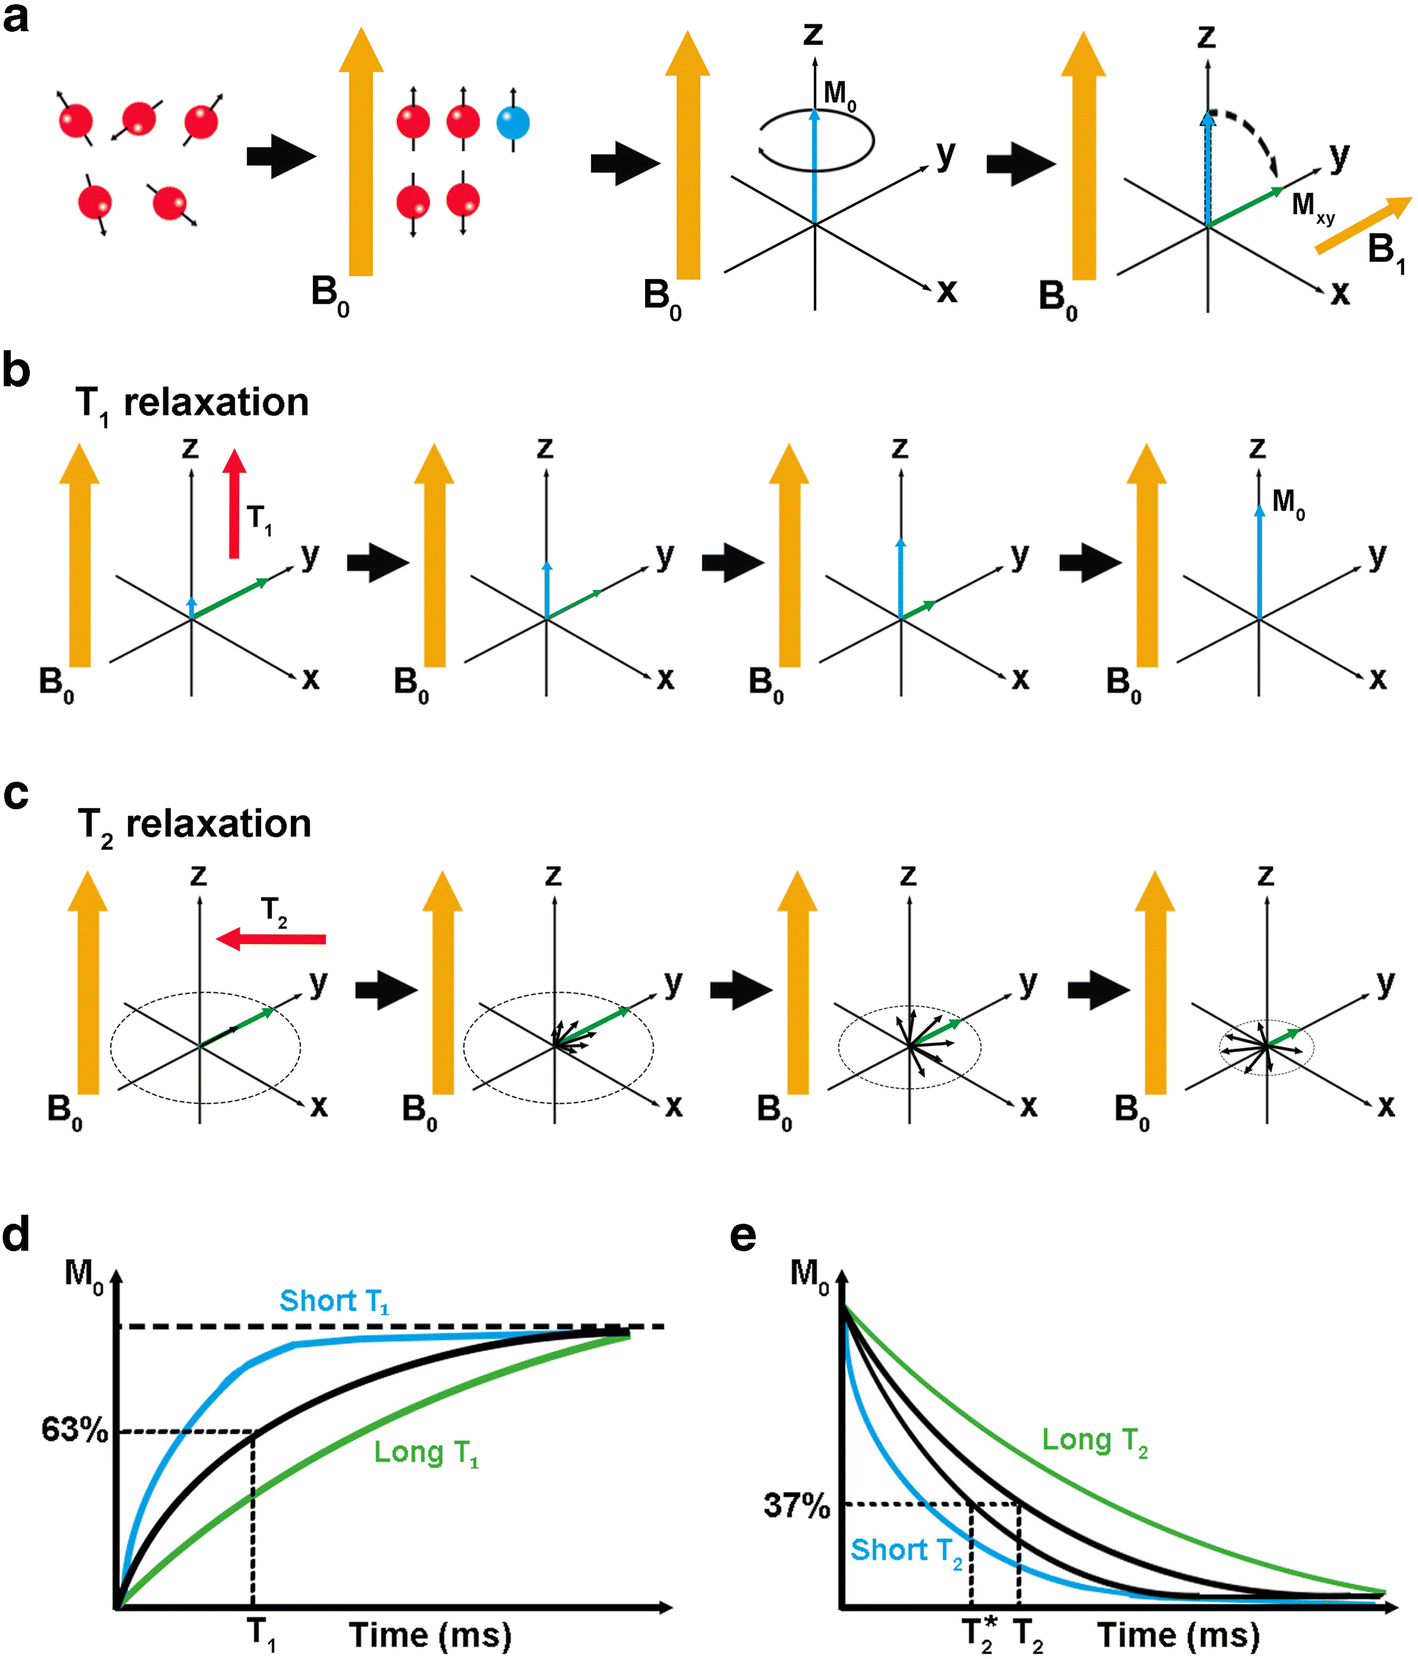
\includegraphics[width=0.8\textwidth]{images/mri1.png}
\caption{figure from \cite{Mastrogiacomo2019}. (a) At first the magnetic moments of the individual nuclei are oriented randomly and cancel out each other, in the presence of an external field $B_0$ they gain a net magnetization, with the presence of the external RF pulse the phase of the net magnetization is changed and magnetic resonance is said to occur. (b) Describes process of T1 relaxation. The value of the T1 constant is the time required to achieve 63\% of the longitudinal magnetization. (b) Describes T2 relaxation. The time constant T2 is the time required for the magnetization to fall to 1/e of its value.}
\label{mriphysics}
\end{figure}

When a radio wave is added to the static field using a radio frequency coil (RF coil) at the Larmour frequency (eqn. \ref{larmour}), termed as $B_1$ in \ref{mriphysics} part a, the direction of the magnetization vector gets altered i.e. ‘flipped’ or ‘tipped’ out of alignment with $B_0$ towards $B_1$ with the angle of rotation being termed as the flip angle. The RF pulse causes exerts torque. Mathematically, the torque can be expressed as
\begin{equation}
    \Vec{\tau} = \Vec{m} \times \Vec{B_1}
\end{equation}
where $\Vec{m}$ represents the magnetic moment and the $ \Vec{B_1}$ is the applied magnetic field.
 The flipping does not bring all the spins in phase with each other but the net magnetization gets flipped ($M_{xy}$) onto the transverse plane. The magnetization $M_{xy}$ precesses 

The net magnetization does not precess until an external force disturbs its equilibrium position of alignment with the static magnetic field. Thus, when the magnetization precesses, magnetic resonance is said to occur. The magnetization has an effect in which the frequency is proportional to the applied static magnetic field.

After this, the RF pulse is switched off which causes the tissue molecules to return to their original state and is termed as the relaxation phase. The relaxation is due to the release of electromagnetic energy into the environment to attain thermal equilibrium. This release of electromagnetic energy is what forms the signal for the receiver coil. \cite{PhysRev.70.460} introduced two time constants to measure the relaxation phase, T1 and T2.

The constant T1  measures the growth of the longitudinal component  ($M_z$, Fig. \ref{mriphysics} part (b) with T1 relaxation being termed as the process by which the net magnetization aligns itself with the direction of the original magnetic field. The T2 constant measures the decay of the transverse component of the magnetization(Fig. \ref{mriphysics} part (c)). The value of T2 reflects the time required for the magentization to fall to $\frac{1}{e}$ or 37\% of its original value, reflected in fig. \ref{mriphysics} part e. Since inside the MRI scanner there can be imhomogneties, another constant $T2^*$ is measured as the T2 time observed while taking the recording.
During the resonance phenomena, the magnetization has components in different directions which can be expressed in terms of the time constants and current time
\begin{equation}
    M_x(t) = M_o e^{\frac{−t}{T2}} \sin{ \omega t}
    \label{mx}
\end{equation}
\begin{equation}
    M_y(t) = M_o e^{\frac{-t}{T2}} \cos{\omega {t}}
    \label{my}
\end{equation}
\begin{equation}
    M_z(t) = M_o (1 − e^{{\frac{−t}{T1}}})
    \label{mz}
\end{equation}
Where $M_x$ ,$M_y$, $M_z$ are the magnetizations along the x,y and z directions and $M_0$ is the magnetization induced by the applied static magnetic field $B_0$. From the equation \ref{mz} it is clear that the T1 constant measure the time required to gain the original magnetization, i.e. when $t=T1$
$M_z = M_0$ and when $t=T2$, $M_{xy} = \frac{M_0}{\cos{\omega T2}}$


T1 weighting is generated on the basis of controlling the repetition time (TR) in a sequence. The TR is defined as the time taken between sucessive excitations of the same region. Using a small TR causes the net magntizations aligned along the fileds to not fully recover. Different brain tissues have different T1 values.  Short T1 times are seen in fat molecules because the complex structure of the saturated molecules leads to flexions and roations which might occur at the Larmour frequency, thus making it easier to return to the initial state, while longer T1 times is observed in comparatively freely diffusing mediums sch as cerebrospinal fluid (CSF). The fat molecules appear bright on the T1-weighted images while liquids such as cerebrospinal fluid appear dark due to longer T1 times.

Similarly, T2 weighting of an image is generated on the basis of echo time (TE). The echo time measures time between excitation and signal measurement. A well adjusted, long TE gives rise to contrast of signals from different images. Fat molecules appear lighter on T2-weighted images due to short T2 time while the cerebro-spinal fluid appears bright since the CSF has long T2 times.


\subsection{Image formation}

An MRI scan needs to represent the 3D nature of the body part under study. Inside an MRI scanner, the gradient coils are hence used to alter the magnetic field along the different spatial directions so that different slices of the subject’s body resonate at different frequencies. The signal is then received by receiver coils that detect only the transverse magnetization. The signal needs spatial encoding since information about the millions of voxels in the brain has to be maintained.

\begin{figure}
    \centering
    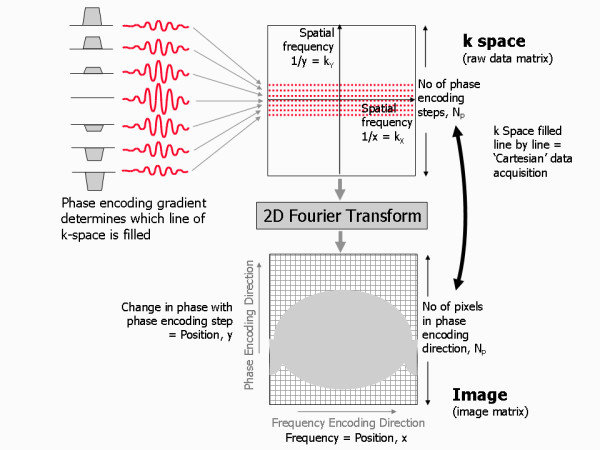
\includegraphics[width=\textwidth]{images/img_reconstruction.jpg}
    \caption{Image from \cite{MRIrecon} summarising the reconstruction of an encoded MRI signal in 2D, after a slice has been selected using the gradient $G_z$. The phase is encoded along the y direction. Each phase encoding step is used to populate the k-space and the number of such steps determines the number of pixels in the y-direction. The frequency is encoded along the x direction. The relationship between the k-space points and the points in reconstructed image space is such that $k_x =1/x$ and $k_y= 1/y$. Each line parallel to the $k_x$ axis corresponds to a separate MRI signal. Each line parallel to the $k_y$ axis corresponds to the amplitude and duration of the phase encoding direction at each phase encoding step.}
    \label{fig:mri_img}
\end{figure}

For the image formation, we know that the magnetic gradients are applied in the x,y,z directions (in order to get the 3D image). This formalism results in each voxel possessing a different Larmour frequency, termed as spatial encoding. 
\begin{equation}
        \label{eq:larmour_grad}
          \omega = \gamma(B_0 + G(x, y, z))
     \end{equation}
       
According to this equation, it is prominent that there is a direct relation between the gradient field and the Larmour frequency. Usually the gradient for the slice selection is applied along the z-direction. For better understanding a simpler case of 2-dimensional image reconstruction has been explained in the figure \ref{fig:mri_img} where the phase encoding gradients are applied in a direction perpendicular to the frequency encoding gradients.

The RF coils in the MRI scanner detects a signal containing a mixture of frequencies specific for each slice and each pahse encoding step. The distribution of frequencies is determined using a Fourier transform. This distribution is then used to fill what is called as the k-space. The 2D k-space in fig. \ref{fig:mri_img} is used to elucidate the components of the frequency . The intensity of a point in the space represents the contribution of the frequency $(k_x,k_y)$ in the signal. For each combination of $(k_x, k_y)$ in the k-space the scanner camera takes only one picture (one filter per voxel) and then estimates the actual intensities at different locations using an inverse Fourier transform. There is a one-to-one correspondence of the pixel in the k-space to the image space, every pixel in the 2D k-space image maps to only one pixel in the reconstructed 2D image but it is not necessary that the locations in both the images are exactly the same. This method is then extrapolated in 3D in order to obtain the image of the whole organ such as the brain. Any weighting, T1 or T2 can then be given in order to generate the image.

Another important concept is that of Field of View (FOV) refers to the distance over which an MRI signal is acquired or displayed. The defined FOV determines the pixel width (determined by the phase encoding y-direction in Fig. \ref{fig:mri_img}), $\Delta k = 1/FOV$. 



\subsection{Diffusion MRI}
Diffusion Magnetic resonance imaging is an \textit{in-vivo}, non-invasive imaging modality that used to create high-resolution structural images of biological tissues. It measures the non-homogeneity of water diffusion in tissues to probe their microstructure (\cite{ghosh2015survey}). One of the most important applications of dMRI is to map the white-matter fiber tracts in the brain. As compared to other MRI techniques such as functional Magnetic Resonance Imaging it does not suffer from an issue of low resolution and low signal-to-noise ratio (\cite{wong2016}). 

“Diffusion” is defined as the net movement of a substance from a region of higher concentration to a region of lower concentration. In a homogeneous medium, the diffusion of water molecules is isotropic, i.e. they can move in any direction with equal probability or exhibit random walk behavior explained by Brownian motion (\cite{Brogioli_2000}).
The environment inside a biological tissue is complex and the diffusion of water molecules becomes anisotropic due to the hindrances imposed’ by cellular membranes. Water molecules in the extracellular environment hence experience relatively free diffusion and the ones in the intra-cellular environment experience restricted diffusion (\cite{toennies2017guide}). This diffusion anisotropy is encoded into the MRI signal using spatial and temporal variation(gradients) in the magnetic field (the alignment of the molecules which have different diffusion hence becomes different). The MRI signal is said to be “Diffusion Weighted” due to the signal attenuation introduced by the magnetic field gradients. 


\subsubsection{Diffusion Weighted Imaging}
\label{DWI}
In this type of Diffusion imaging, the intensity of each voxel represents the rate of water diffusion in a cubic region. Diffusion weighting is applied in order to generate contrasts based on the presumption that diffusion varies with pathology i.e. differences in diffusion can also highlight differences in structure and function (\cite{Taylor_1985}). 

One of the most popular ways to give images Diffusion weighting is through using single-shot-spin-ehco (SE) T2 weighted sequences with two symmetric gradients on each side of the 180 degree refocusing pulse. This is based on the pulsed gradient spin echo (PGSE) technique developed by (\cite{stejskal1965spin}) in the mid 1960's, which resulted in much improved sensitivity to diffusion in comparison to the steady state gradients used previously. They solved the Bloch-Torrey partial differential equations for a symmetric pair of pulsed gradients and obtained the well-known Stejskal-Tanner formula
\begin{equation}
\label{eq:Stetjskal}
S = S_0 \exp^{-bD}
\end{equation}
\begin{figure}
    \centering
    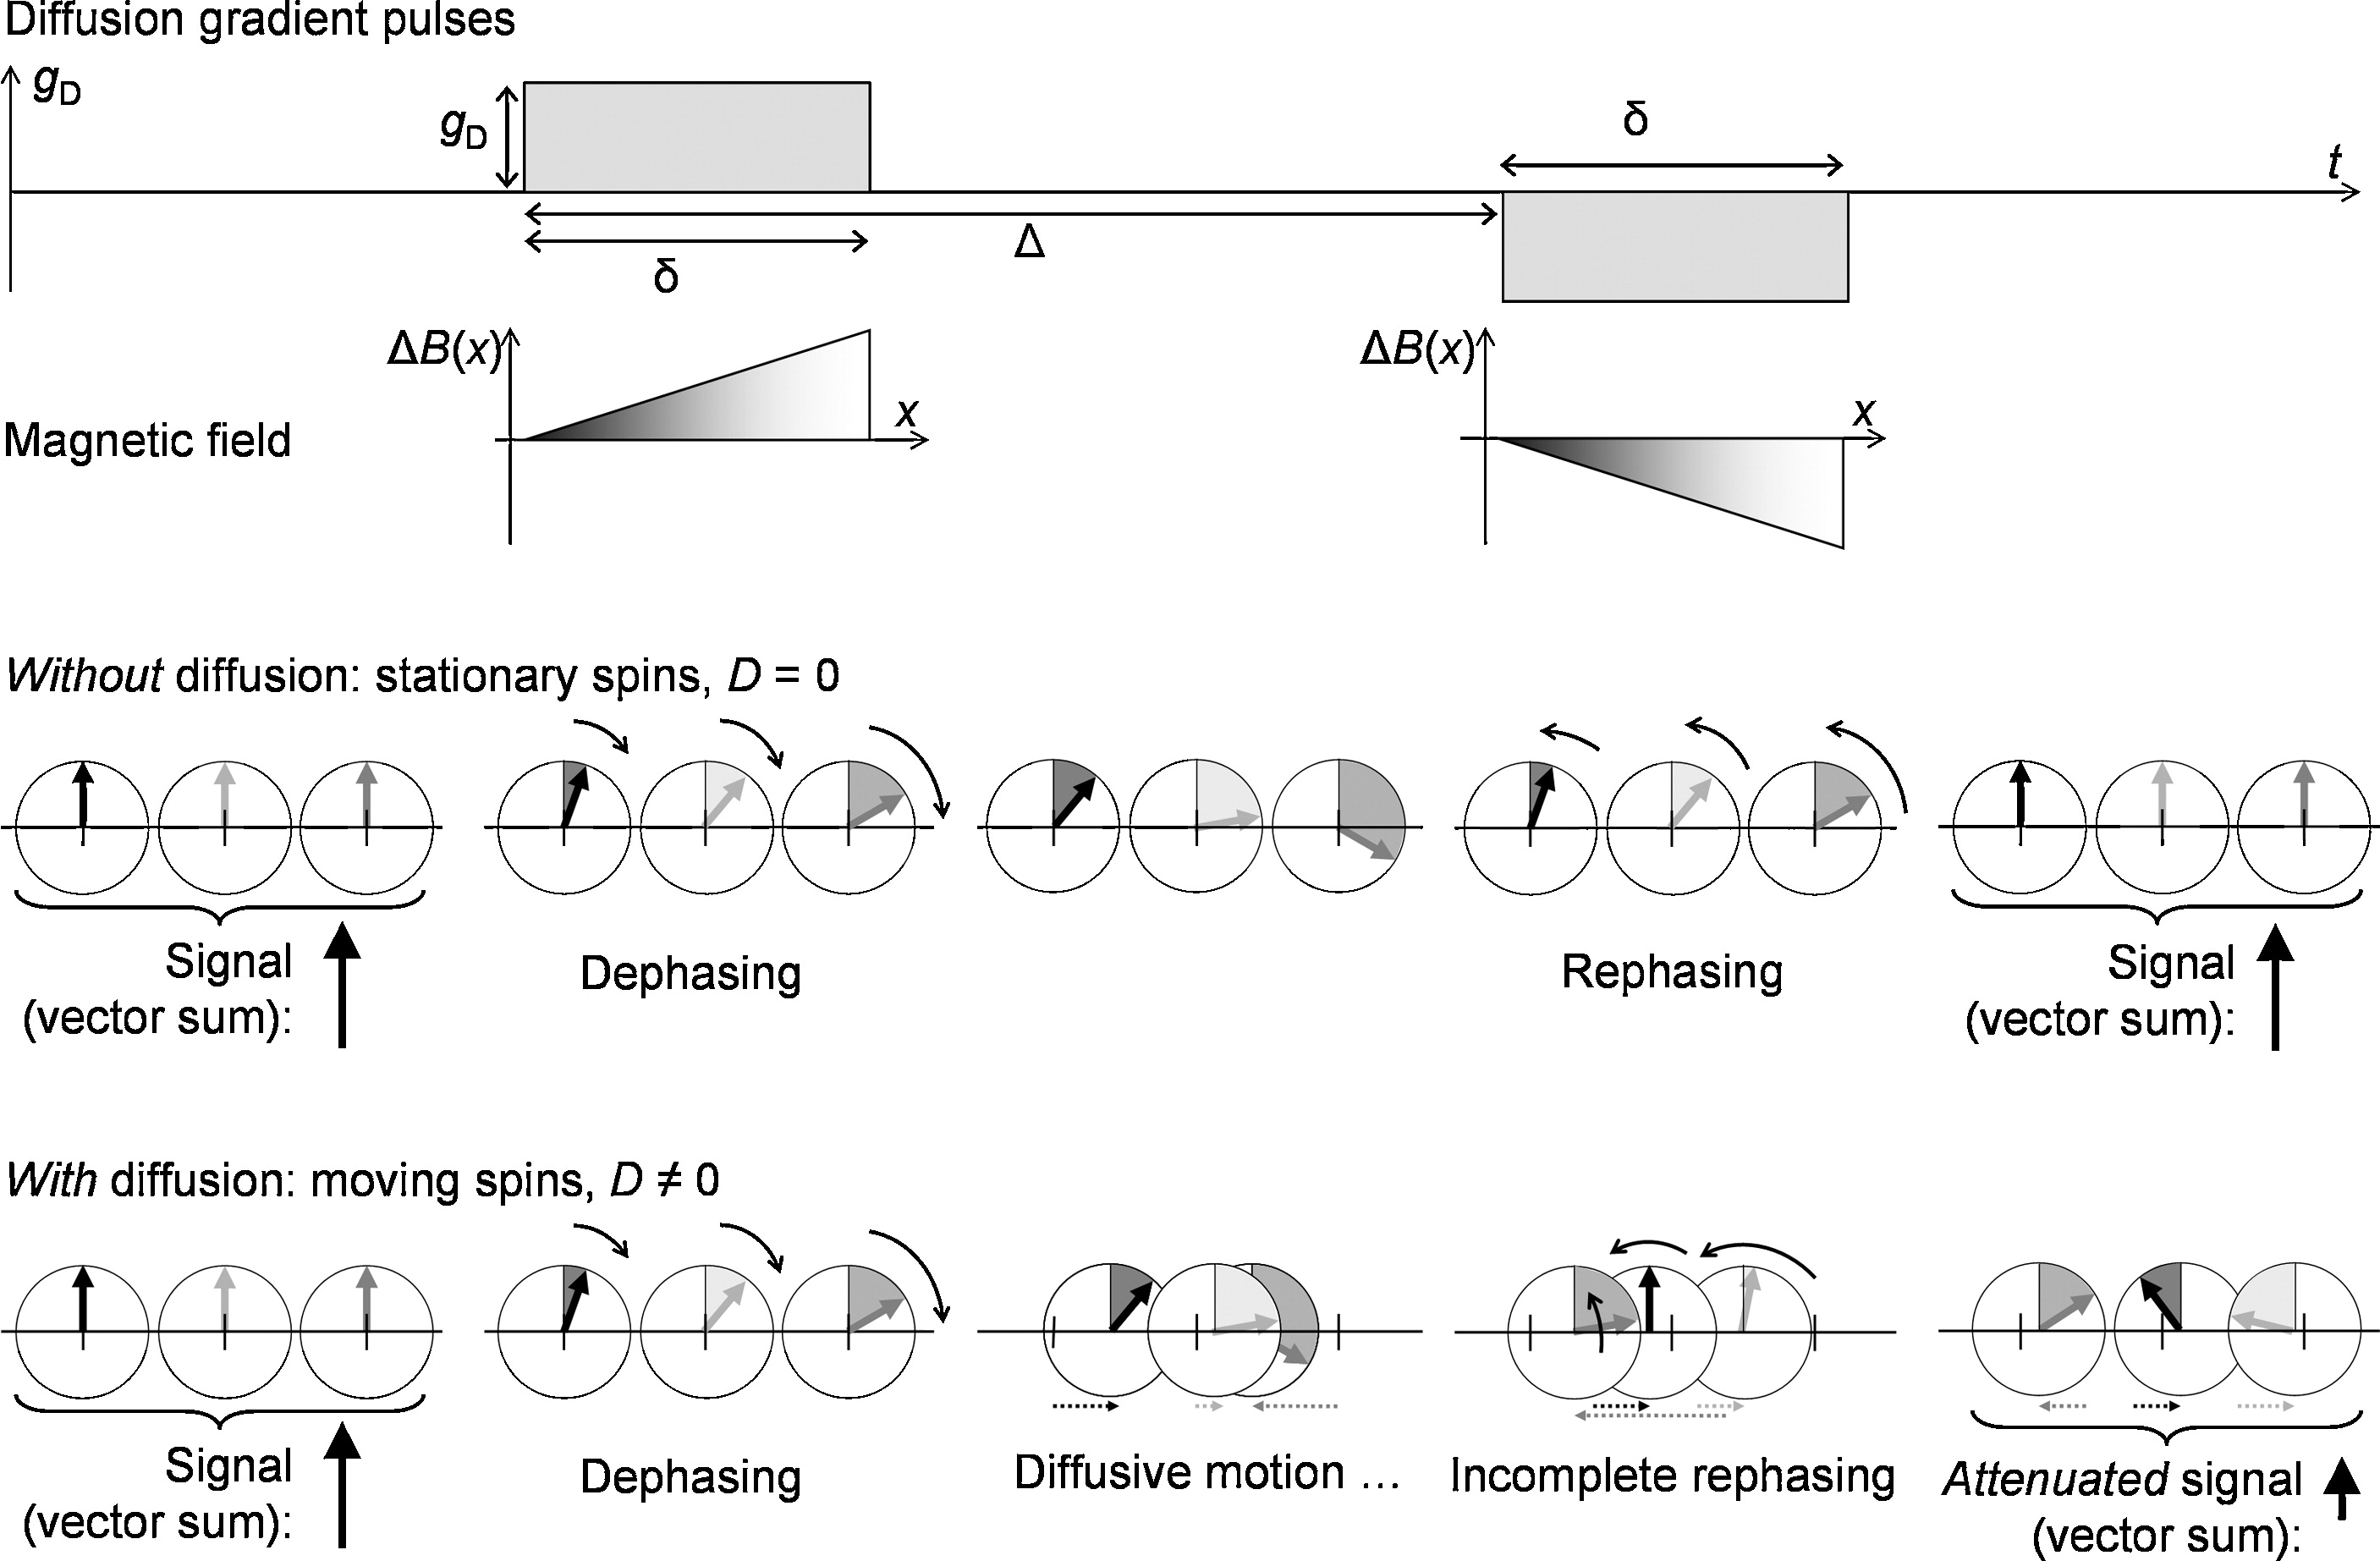
\includegraphics[width=\textwidth]{images/diffusionmri.jpg}
    \caption{Image from \cite{technical_aspects_dmri} elucidating the technical aspects of Diffusion Weighted MRI. The RF pulse causes a phase change of the magnetization. Introducing the diffusion gradient adds spatial dependence of phase shift of the individual magnetic moments. The molecules that have restricted diffusion remain along do not experience the effect of the diffusion gradient, any phase change from the first gradient is reversed by the second,  and tend to relax to their equilibrium state. However, molecules that undergo free diffusion experience the effects of the diffusion gradients introduced by the second RF pulse (180 degrees) and hence will undergo a total phase shift dependent on the spatial location, this phase shift is then manifested in terms of signal attenuation.  The degree of signal attenuation depends on multiple factors as shown in the following equation: SI0 is the signal intensity of the T2-weighted image with no diffusion gradient applied, b is the degree of diffusion weighting (b value), and D is the diffusion coefficient  }
    \label{fig:diffmri}
\end{figure}

$S_0$ represents the original signal strength,  $S$ is the signal strength in a pulse sequence with the presence of diffusion gradients ($g_D$) and $D$ represents the diffusion coefficient. The the attenuation of the diffusion MRI signal by the diffusion gradients is represented in figure \ref{fig:diffmri}. The application of the Diffusion gradient results in a spatial encoding as the Larmour frequency is dependent on the net magnetic field (equation \ref{eq:larmour_grad}). In the figure \ref{fig:diffmri}, it is evident that the Diffusion gradients are magnetic field gradients along the x direction. 
Here $\Delta B_(x) = g_D x$ which makes the Larmour frequency spatially dependent $\Delta \omega = \gamma \Delta B_(x)$ or $\Delta \omega = \gamma g_D x$. There is a phase shift introduced after the gradient pulse of time duration $\delta$. The the phase shift is also dependent on the x position due to the spatial dependence of $\Delta w(x)$  ,  the phase shift is $\Delta \phi (x) = \Delta w \delta = \gamma g_D x \delta$. This spatial dependence of the phase shift makes spins at different positions along the gradient axis "dephased" after the application of the gradient pulse. When the negative gradient is applied, the process of rephasing occurs. The dephasing and rephasing mechanisms result in the Diffusion weighting of the image, without any diffusion stationary spins would align along their equilibrium position (cancelling effect of the two Diffusion gradients) while with Diffusion weighting there is a signal attenuation explained by equation \ref{eq:Stetjskal}. 

The where the b value of the sequence is defined in the units of $s/mm^2$ as
\begin{equation}
    b = (\gamma g_D \delta)^2 (\Delta - \frac{\delta}{3})
\end{equation}
In order to obtain the numerical value of b, long and strong gradients are required. The diffusion gradients $g_D$, time of pulse $\delta$ and time interval $\Delta$ are often adjusted to adjust the b values. Higher b values leads to lower signal in the areas of high diffusion and increases the contrast between tissues that have different diffusion coefficients. Also, the b values need to be adjusted in order to obtain optimal signal to noise ratio (SNR)


\subsubsection{Diffusion Tensor Model}
Diffusion Tensor Imaging (DTI) is a new type of imaging technique that relies on a tensor model to measure the diffusion among voxels. Instead of attributing diffusion inside a voxel by using a single quantity, it uses a tensor formalism to measure diffusion along different directions within a voxel. The tensor model gives a rotationally invariant description of water diffusion and hence able to trace complex fiber tracts in the brain. (\cite{jones2010diffusion})

Diffusion Tensor Imaging is a novel technology, an \textit{in-vivo } application of DWI that is the gold standard for imaging neural fiber tracts. It has become an important brain imaging modality since various neurological disorders such as cerebral ischemia and Parkinson’s disease can be attributed to defects in white matter. Further, white matter constitutes about 50\% of the brain (by volume) which makes it important to understand both its structure and tissue composition. Analyzing structural brain connectivity or the ‘connectome’ using DTI does not only help to understand the pathophysiological effect of brain disorders but also the structure of functional networks.

In this type of imaging, each voxel is associated with a 3x3 Diffusion Tensor representing the diffusion of water molecules using a Gaussian Model. It is symmetric and contains six unique variables that characterize diffusion (as anisotropic or isotropic). This tensor has 3 eigenvalues and corresponding eigenvectors which represent the directions of Diffusion along the voxel, the voxels are usually 1 mm3 in size and often constitute components of more than one cell within them.
\begin{equation*}
D =
\begin{pmatrix}
D_{xx} & D_{xy} & D_{xz} \\
D_{yx} & D_{yy} & D_{yz} \\
D_{zx} & D_{zy} & D_{zz}
\end{pmatrix}  
\end{equation*}

where $D_{xy} = D_{yx}$, $D_{zy}=D_{yz}$ and $D_{xz}=D_{zx}$
In this case equation \ref{eq:Stetjskal} can be written as 
\begin{equation}
\frac{S}{S_0} =  \exp^{-bg^T Dg}
\end{equation}where $g^T$ is a 3x1 unit vector representing the gradient direction.
The cellular environment is heterogeneous, so water molecules in certain parts undergo free diffusion while in others they undergo restricted diffusion. Due to this restricted diffusion the measured diffusion coefficient (of the water molecules) is different from the regular diffusion coefficient of water, it is termed as the “apparent diffusion coefficient”. Diffusion in complex environments cannot be explained by using diffusion gradients in one direction only. In fig \ref{fig:diffmri} of the Diffusion Weighted MRI, only the component along the gradient direction is detected. Therefore, it is required to apply diffusion gradients in three directions to get an estimate of anisotropy of water molecules hindered/interacting with cell membranes/extracellular environments. 

DTI images are usually represented by either encoding the tensor information using a scalar (for intensity values in a black and white image) or 4 numbers (R,G, B and brightness). Visually, the tensors can also be viewed as glyphs and very famously by tracing white matter tracts through a process known as tractography.


There are three important quantities that can easily be derived from the diffusion tensor. These help to analyze the nature of differences in diffusion along the various voxels of the image. The three quantities are mean diffusivity, diffusion anisotropy and fractional anisotropy. The trace of the Diffusion tensor is used as Mean diffusivity. While the diffusion anisotropy exhibits the deviation of the voxel diffusion from isotropic diffusion; high diffusion anisotropy means that there is a preferred direction for the water molecules within that voxels to diffuse (an indication of more white matter?

The fractional anisotropy determines a sort of average ratio of diffusion distortion from the applied gradient directions. In order to calculate the FA, the diffusion tensor is converted to a diagonal matrix (which has eigenvalues D1, D2,D2 the diffusion coefficients along xx,yy,zz) \\
\begin{equation*}
D =
 \begin{pmatrix}
D1 & 0 & 0 \\
0 & D2 & 0 \\
0 & 0 & D2
\end{pmatrix}   
\end{equation*}


\begin{equation}
FA = \sqrt{\frac{3}{2}} \frac{\sqrt{(D1 -D_{mean})^2+(D2 -D_{mean})^2 + (D3 -D_{mean})^2
}}{\sqrt{D1^2 + D2^2 + D3^2}}
\end{equation}


Where D1, D2, and D3 are the corresponding eigenvalues and v1,v2,v3 are the eigenvectors.
DTI is a popular method to study the orientation and organisation of white matter. However, its fails in regions containing populations of fiber orientations that have different orientations. It assumes that all white matter bundles in the brain have similar diffusion characteristics and attributes diffusion anisotropy to partial volume effects \cite{tournier2004direct}. Secondly, the Diffusion tensor only possess a single major eigenvalue for modelling the diffusion in one voxel and cannot be used for mixed fiber populations.
\subsubsection{Higher order models}

In order to solve the multiple fiber orientation problem in DTI, a number of approaches have been proposed to estimate the composition of fiber orientations inside a voxel. These models extract higher order structural information of tissues. They can help deal with probelms of kissing fibers/crossing fibers etc.

These rely on the concept of an fiber orientation distribution function (fODF)
An fODF is a symmetric probability distribution function describing the distribution of fiber orientations
\begin{align}
  F(\Theta, \phi) = \sum_{k=1}^{K} w_k \delta_{\theta_k, \phi_k}(\Theta, \phi) &
 & \Theta \in [0, \pi], \phi \in [0,2\pi]
\end{align}
where $w_k$ represents the volume fraction of each fiber passing through the voxel. $\Theta_k$ and $\phi_k$ represent the polar and azimuthal angles in spherical coordinates respectively.

High angular resolution imaging (HARDI) techniques enable the detection of multi-modal diffusion signals. Q -ball imaging is one such technique but has its own limitations \cite{TOURNIER20041176}.

The DWI signal is modelled as the spherical convolution (i.e. convolution in spherical coordinates) of the response function and the fODF. Spherical deconvolution is the other way round where fODF can be extracted.

Constrained Spherical Deconvolution (CSD) has gained recent attention as a method to extract white matter (WM) fibre orientation distributions. It is used to obtain fODF estimates and fibre tractograms \cite{JEURISSEN2014411}.


\subsection{Tractography}
\label{sub:tractography}
\begin{figure}
    \centering
    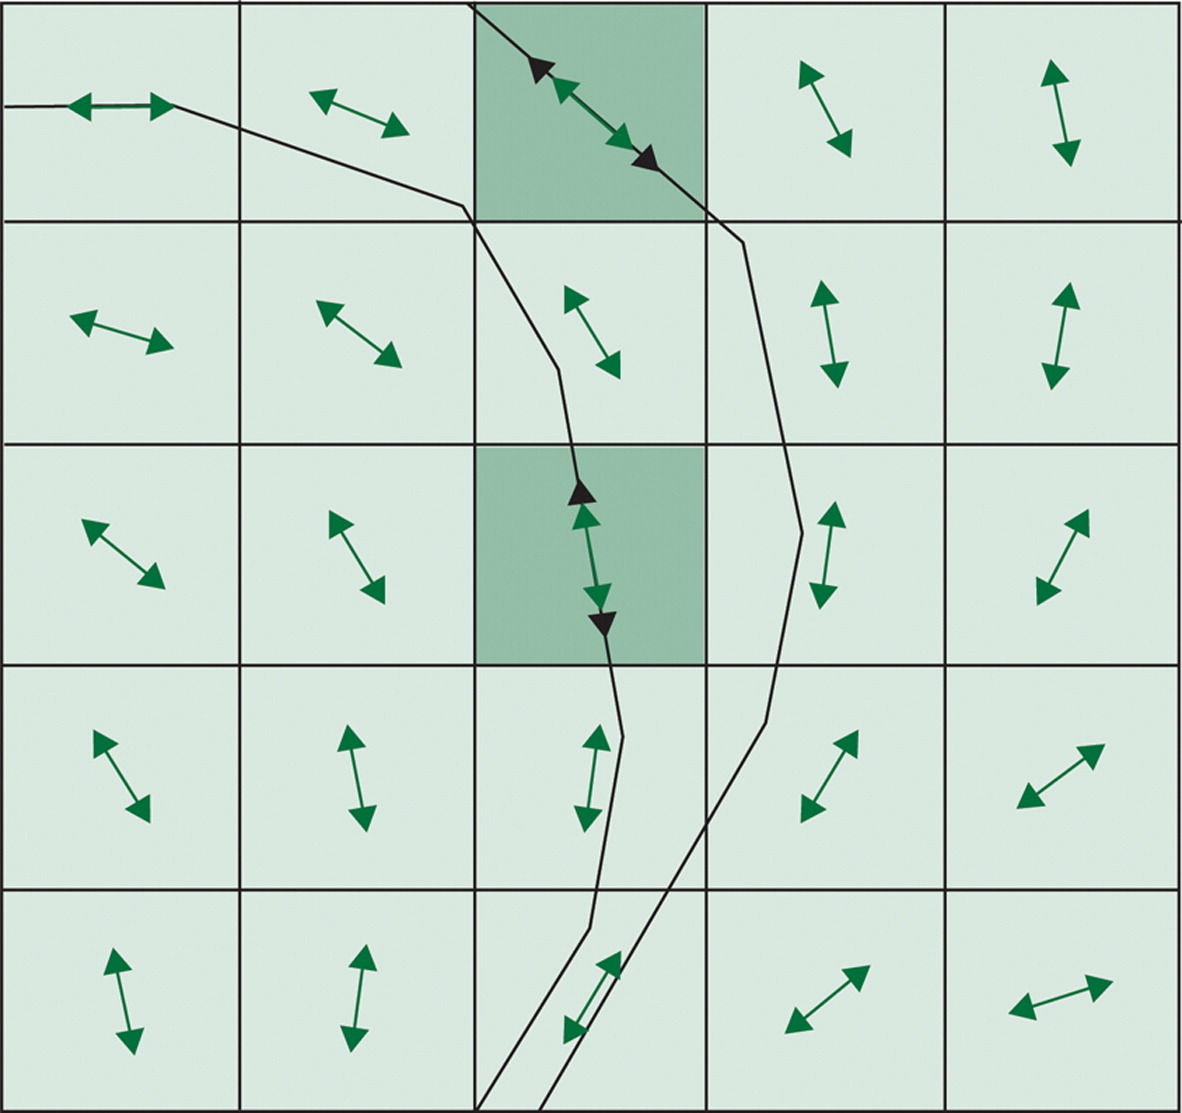
\includegraphics{images/fibertracking.png}
    \caption{Deterministic tractography from }
    \label{fig:tracking}
\end{figure}
Fiber tractography is a technique used to graphically construct  3 dimensional representations white matter pathways in the human brain.The technique uses the information about local fiber directions to trace streamlines that represent white matter tracts in the brain. It has become an important part of white matter disorder studies and has gained popularity because of its non-invasive nature. These advantages make it suitable for surgical targeting and planning \cite{romano2009pre}.

Tractography methods often use DTI in order to delineate the streamlines along the white matter tracts by getting the information about their progression from one voxel to the next. This methodology relies on the assumption that the direction of maximum diffusion(in the diffusion tensor) aligns with the direction of the white matter fiber within the voxel. 

In deterministic tractography, the algorithm usually follows the direction of maximum diffusion from along the voxels by starting from a “seed” region. If the angle between two subsequent directions of maximum diffusion is less than predefined threshold then the algorithm proceeds tracking along the maximum diffusion direction of the second voxel and terminates when the condition is not met \cite{}.  Several other conditions can also be imposed on the basis tracking technique on the basis of investigator specific techniques. The deterministic tractography does not take into account any random or systematic errors that arise during signal acquisition, recording and transmission.



\section{Connectomics}
\label{sec:connectomics}
Connectomics is termed as the study of the brain's functional and structural networks. A connectome (in-vivo, retraced from imaging) is a dense network of brain connections, with a numerical value assigned to each network (\cite{bassett2017network}). The connectome of brain can be seen as a circuit diagram with the neural connections analogous to wires and the cell bodies to electrical components.
Recently, connectomics has become the focus of major Neuroscience studies with evidence about the hodological view. The research in the field has expanded rapidly due to the increasing interest in understanding the brain as a dynamic system, and the belief that the connections in the brain are what give it its capabilities and functionality. \cite{network_neuroscience_editorial}

The first complete structural connectome to be mapped at the synaptic level was published in 1986,  belongs to the species C. elegans. It was reconstructed using electron micrographs of serial section and is a network that possess three hundred neurons and roughly seven thousand connections. It still took decades to claim the biological plausibility of all the connections in the reconstructed connectome\cite{elegans}, this leads to the fact that the connectome of the human brain cannot be mapped using the manual labour intensive methodology used by \cite{white1986structure}. Mapping the human brain manually seems implausible. The human brain contains roughly the same number of neurons as the stars in the Milky way galaxy and about $10^{15}$ inter neuronal connections (synapses)\cite{fornito2015connectomics}. This calls for the need to computationally determine brain connectivity from brain scans. dMRI and functional MRI are the preferred modalities for connectome construction. The Human Connectome Project was launched in 2007 as the first large scale collaborative effort to create detailed maps of the brain (in-vivo) and to help better understand the fundamentals of human connectional anatomy.

\subsection{Structural Brain Connectivity}
%the term connectivity refers to several different and interrelated aspects of brain organization (Horwitz, 2003)
% is the anatomical connectivity in the brain
Structural brain connectivity refers to the arrangement of anatomical connections in the brain. A model of the brain's structural connectivity can derived from whole brain tractography.In organisms such as humans with complex nervous systems, the structural brain connectivity can be visualized at different scales. It can be either at the level of synaptic connections (microscale), at the level of neuronal populations (meso-scale) or at macro scale in which fiber tracts run between different brain regions. At all these scales, the connectivity patterns of individuals from the same species exhibit different characteristics such as organization, topology and spatial extent (\cite{Sporns:2007}).

Usually in Neuroimaging studies the connectivity is analyzed at the macroscopic scale, i.e. the running of the fibers between different brain regions.  From section \ref{subsub:tractography} it can be inferred that the streamlines traced using the tractography algorithms represent the structural connections between different Regions of Interest(ROIs) of the brain. The connections are usually represented using bio-physical parameters such as mean FA (mean fractional anisotropy), number of streamlines between the two nodes and the length of the streamlines connecting the two nodes.

\subsection{Analyzing the brain as a graph}
A graph can be defined as mathematical representation of pairwise relationships between objects. A graph is said to consist of two basic elements i.e. nodes (representing the objects themselves) and edges (representing the relationships between the nodes). Graph theory can be defined as a branch of discrete mathematics that deals with the geometric analysis of graphs. Graph theory is useful in the analysis of biological networks since biological systems are dynamic and the interaction between the elements of the network gives rise to emergent properties which can only be deciphered by comprehending the behavior with a systems approach. Hence, using graph theoretic methods to infer from dense graphs derived from structural brain connectivity is useful for exploring properties related to the knowledge we want.  

As per the definition of a connectome mentioned in \ref{sec:connectomics}. In this case it empirical to use coefficients or parameters that represent the information about the connectivity, so graph theory is applied to  get the topological properties along with ......To analyze such characteristics, the brain can be seen as a dense graph where the connections represent the edges and the brain regions represent the nodes.
\iffalse
The structural networks in the brain have emerged from many years of evolution to guide effective function and coordination, now that the localized view (that we can define regions of interest in the brain, which are anatomically and/or functionally distinct)
\fi

\section{Feature Selection Techniques}
Neuroimaging data often suffers from the \textit{curse of dimensionality}. The sample size is often much smaller than the total number of features. Classifiers might be influenced by the increase in noise as the number of features increases. Dimensionality reduction and feature selection are often the techniques used for a meaningful reduction in features. Hoewever, most dimensionality reduction methods such as Principal Component Analysis (PCA) rely on transformations (often non-linear) of the original data and this leads to a lack of interpretability. Due to this reason it is important to consider feature selection methods where inference about what the classifier actually learns can be made (\cite{shi2018feature}). 

Feature selection methods can be grouped into three types; filter methods, wrapper methods and embedded methods. Filter methods are based on selecting features before running the classifier. Wrapper methods can be seen as a selection method \textit{on the fly} in which features are added or removed iteratively on the basis of classification performance.Embedded methods are those in which feature selection is embedded in the classifier. These have been increasingly used in Neuroimaging studies \cite{tohka2016comparison}.

\subsection{Filter methods}
Filters form one of the simplest methods for feature selection. They usually serve as a pre-processing step for the classification and are model independent. Hoeever, there is a caveat when using these type of features for classification studies that each feature is considered independently and their cumulative effect is not taken into consideration for the cla
Some of the common techniques used to determine the feature importance is the use of coefficients such as the fscore and t-test, these are also used in Neuroimaging applications. 

The fscore can be calculated as 
\begin{equation}
\label{eq:fscores}
    F = \frac{(\overline{x_{1}} - \overline{x})^2 + (\overline{x_{2}} - \overline{x})^2}
    {\frac{\sum_{i=1}^{n1}(x_{1,i} - \overline{x_{1}})^2}{n_{1} -1} + \frac{\sum_{i=1}^{n1}(x_{2,i} - \overline{x_{2}})^2}{n_{2} -1}}
\end{equation}
where $\overline{x}$ represents the average for all feature values, $\overline{x_{1}}$ the feature average for for the first class, $n_{1}$ represents the number of samples for the first class and other variables follow respectively.

A simple t-test can also be computed and then the features can be filtered based on the t-statistic or the p-value to test the significance of the differences between the feature values for two different groups. Based on \cite{inza2004filter}, the t statistic is calculated as:
\begin{equation}
    t = \frac{|\overline{x_1} - \overline{x_2}|}{\sqrt{0.5(\sigma_{1}^2 + \sigma_{2}^2)}}
\end{equation}
The features can be ranked and the features with the highest t-test scores can be used to perform the classification. Numerical thresholds can also be imposed if suited to the nature of the problem. 
\subsection{Maximum Weight Subgraph}
In the above section it was presented that the brain can be analyzed as a graph. 

The definition of the maximum weight connected subgraph can be given as 
\begin{equation}
    \Omega(\Tilde{G}) = \sum_{v in \Tilde{V}} w_v + \sum_{e \in \Tilde{E}} w_e \longrightarrow max
\end{equation}

Such a problem is formulated using a Mixed INteger programming formulation. 

The representation is as follows for the subgraph. the variables are
\begin{itemize}
    \item Binary variable $y_v = 1$ iff $v \in V$ and $v \in \Tilde{V}$
    \item Binary variable $w_e =1 $ iff $e \in E$ and $e \in \Tilde{E}$
\end{itemize}
These variables can represent a valid subgraph iff for the constraints be satisfied. 
\begin{align*}
    w_e \leq y_v & \forall v \in \V, e \in \delta_{v}
\end{align*}

For the non-linear formulation the graph can be considered as set of binary variables and continuous variables
\begin{itemize}
    \item Binary variable $x_a = 1$ iff $a \in A$ belongs to the arborescence.
    \item Binary variable $r_v = 1$ iff $v \in V$ is the root of the arborescence,
    \item Continuous variable $d_v = n$ if the traversal from the root of the arborescence to the vertex v goes through n vertices. The $d_v$ value can be arbitrary if the vertex v does not belong to the optimal solution.
\end{itemize}
To ensure the validity of the arborescence the following constraints were introduced. 
\begin{align}
    \sum_{v \in V} r_v = 1\\
    1 \leq d_v \leq n && \forall v \in V \\
    \sum_{(u,v) \in A} x_{uv} + r_v = y_v && \forall v \in V\\
    x_{uv} + x_{vu} \leq w_e && \forall e =(v,u) \in A\\
    d_v r_v = r_v
\end{align}

Linearization of the above inequalities
\begin{align}
    d_v + n r_v \leq n && \forall v \in V\\
    n + d_u - d_v \geq (n+1) x_{vu} && \forall (v,u) \in A\\
    n + d_v - d_u \geq (n+1) x_{vu} && \forall (v,u) \in A\\
\end{align}


\section{Classification}
\subsection{Support Vector Classifiers}
\begin{figure}
    \label{fig:svm}
    \centering
    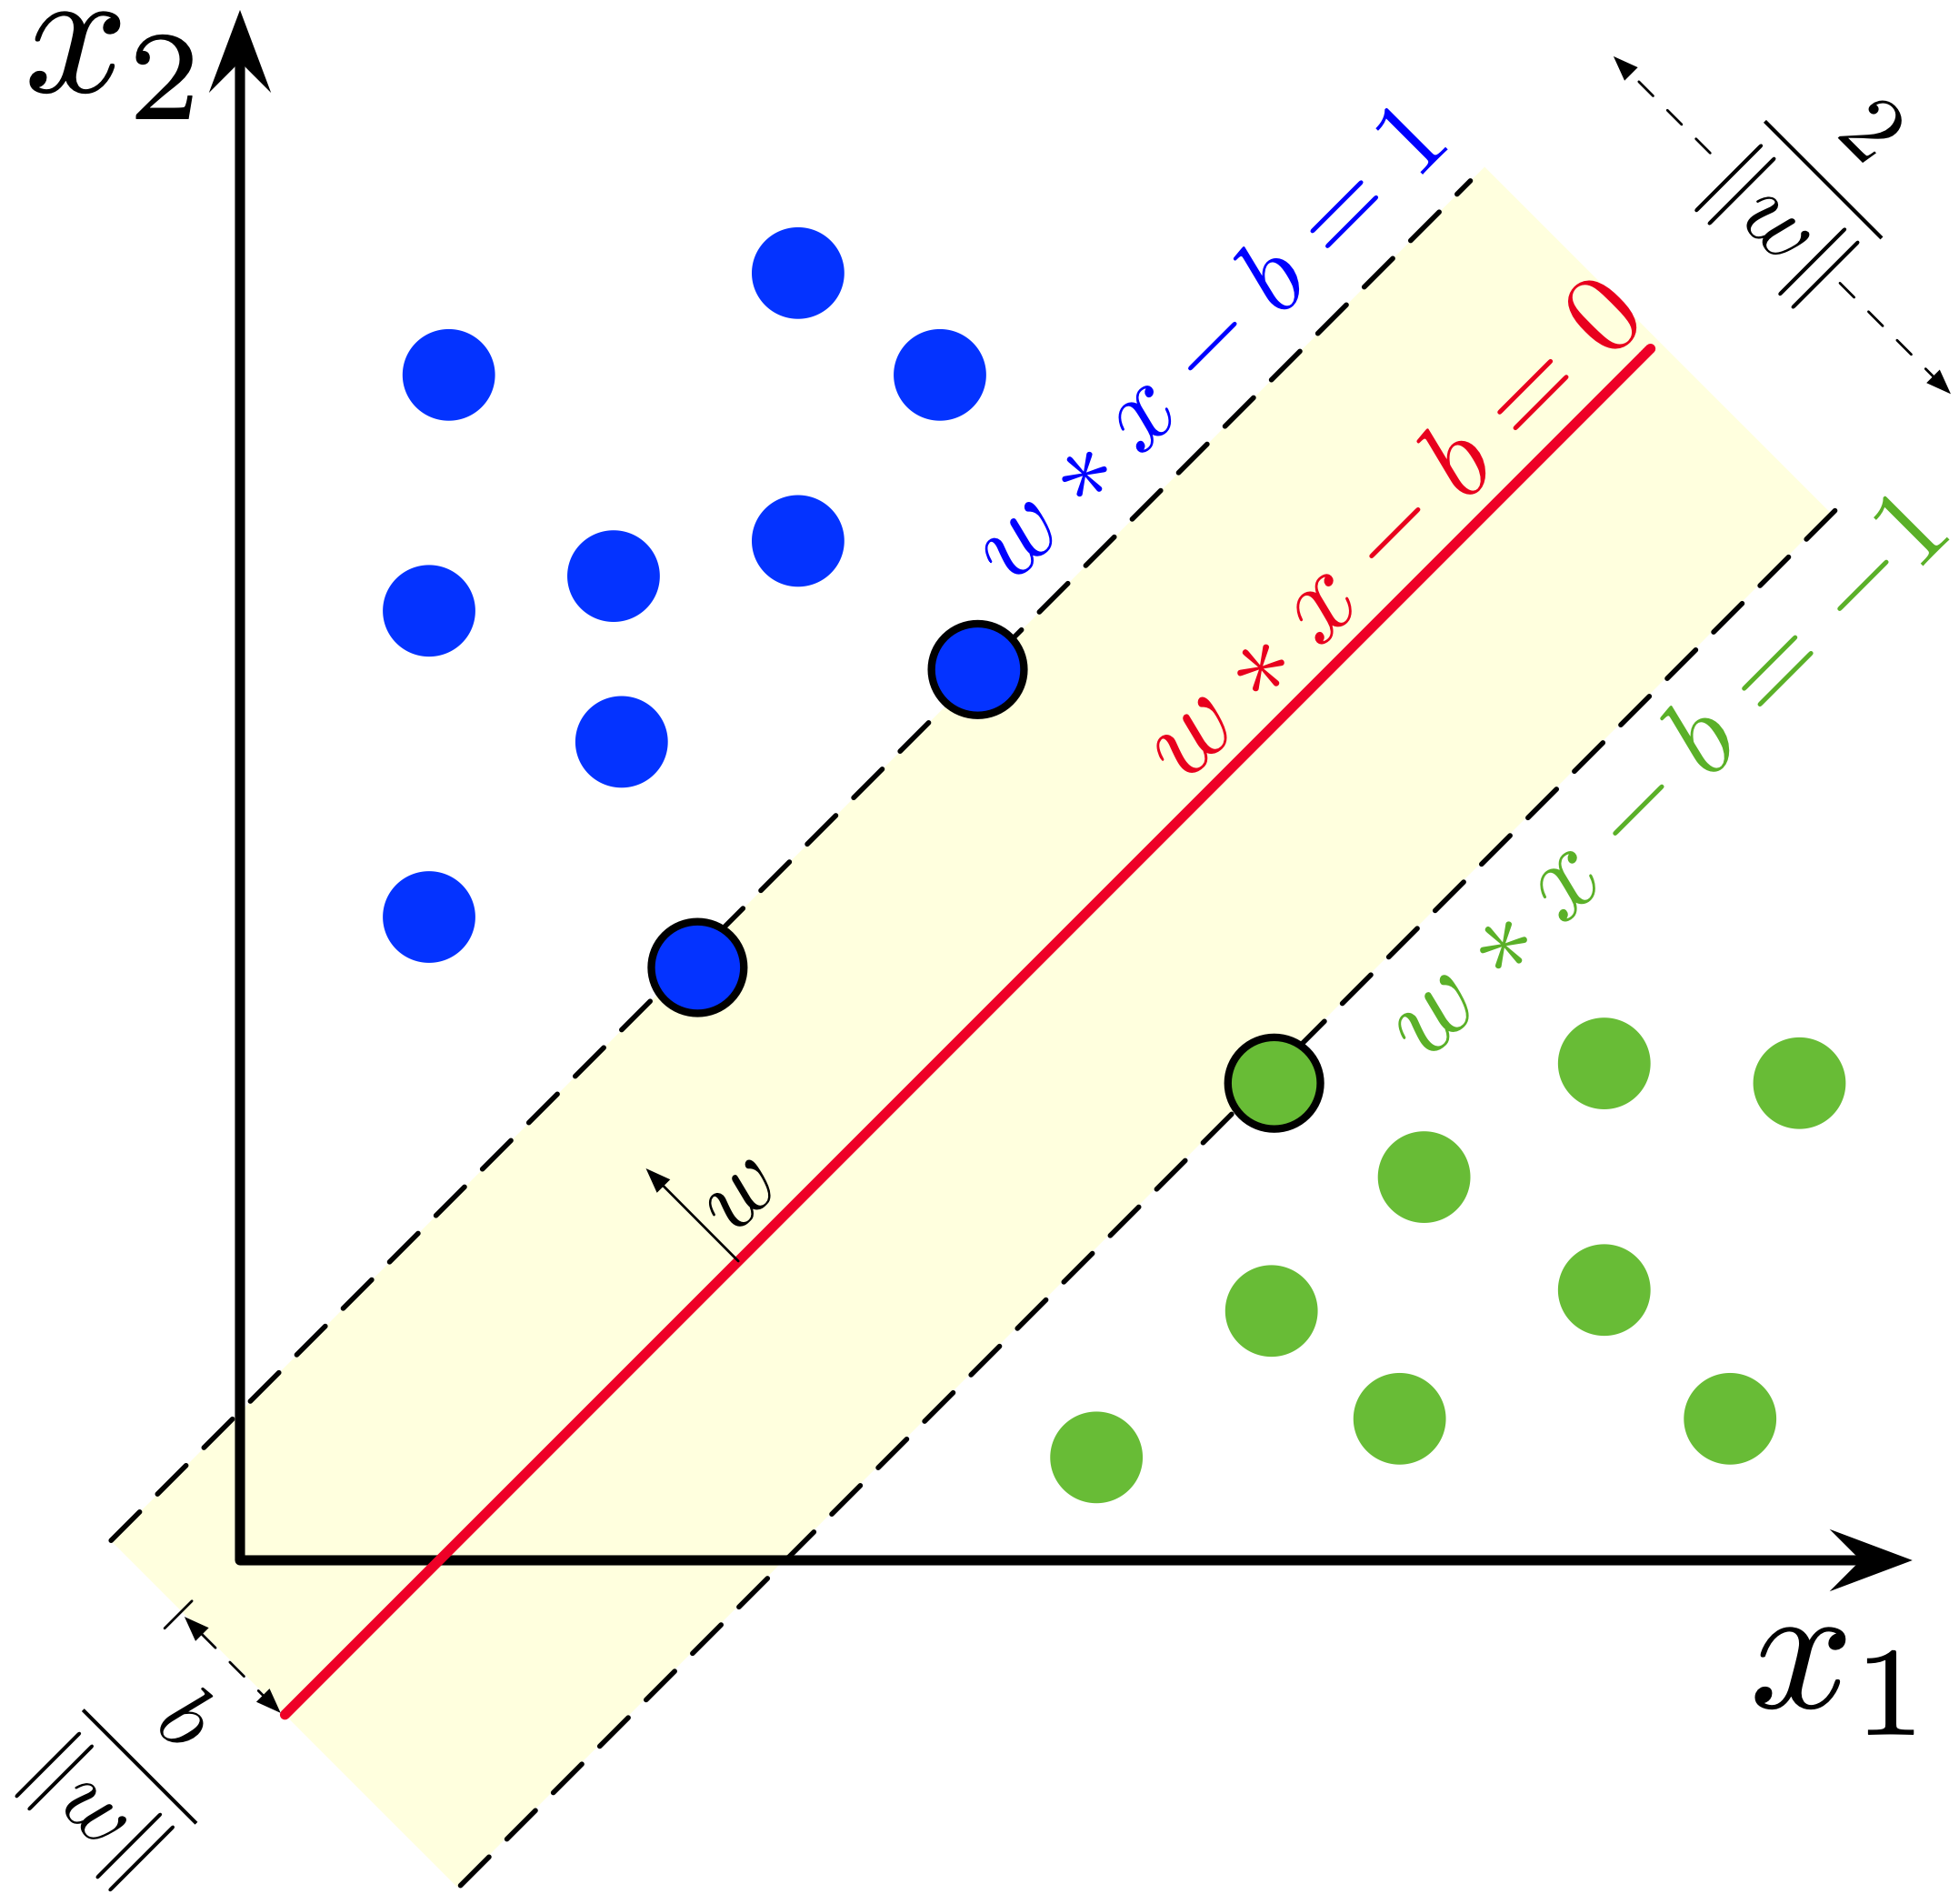
\includegraphics[width=0.4\textwidth]{images/svm.png}
    \caption{Caption}
    \label{fig:my_label}
\end{figure}

Support Vector Classifiers (SVC) are classical machine learning algorithms based on Support Vector machines (SVMs). They are important since they have attained signifcant accuracy with different types of tasks such as a handwritten digits recognition, face detection in images, and text categorization\cite{burges1998a}. In Neuroimaging studies, SVCs are important for classification tasks since they are relatively robust to overfitting and more interpretable than Deep Learning classifiers.

In the simplest, binary case the mathematical formulation of the SVM is as follows. Consider each observation \textbf{$x_i$}, $i\in {1...n}$ to be a vector in the \textit{d-dimensional} feature space with a target label  $y_i\in {-1,1}$. The classifier needs to find a boundary that separates \textit{n} such points present in the presented data within a small margin of error.  It does so by trying to find an optimally separating hyperplane that efficiently divides the input data according to the target labels. In figure \ref{fig:svm} the red line represents the optimally separating hyperplane that satisfies the equation
$ \sum w_i x_i - b = 0$
 It is maximally distant to the nearest point belonging to either class (also termed as the support vectors). The maximally separating hyperplane is found by satisfying the following constraints for each data point i. 
\begin{align}
    y_i(\sum_{j=1}^{d} w_{j} x_{ij}  + b)  - 1\geq 0 && \forall i \in {1...n}
\end{align}
Here, the weights represent the parameters the model learns in order to satisfy the above conditions by solving a Langrangian equation, the mathematics of which is beyond the scope of this text.  

In cases where the decision boundary is a non-linear function of the data the algorithm makes uses of what is commonly called as the 'kernel trick'. In this method the pairwise dot products of the individual $x_i$ are replaced by a non-linear transformation or kernel function. This expression then allows the algorithm to fit the maximally separating/maximum margin hyperplane in the transformed space. The decision boundary is linear in the transformed space and can be projected back to find the non-linear decision boundary in the original $d$ dimensional feature space. 
\subsection{Random Forest Classifiers}
\begin{figure}
    \centering
    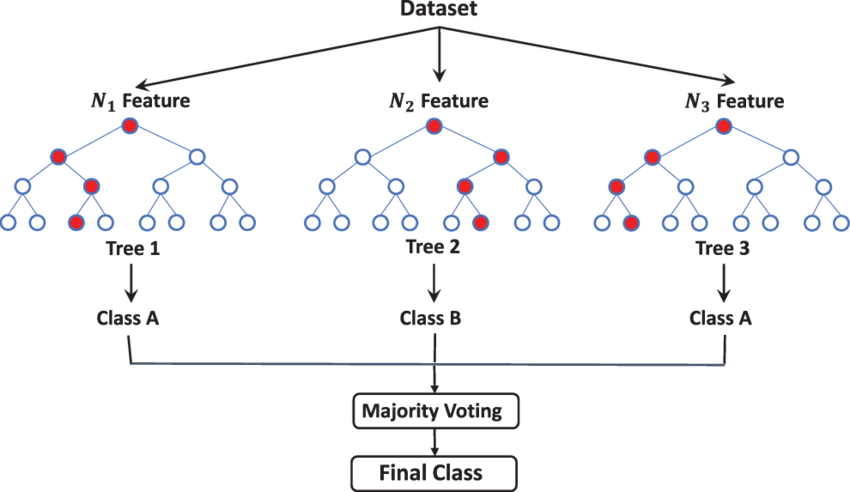
\includegraphics[width=0.8\textwidth]{images/Random_forest.png}
    \caption{Schematic explanation of Random Forest classifier from \cite{TAHMASEBI2020103619}. The different trees represent the decision trees constructed from the bootstrapped samples. Each tree is created on the basis of the most discriminatory features, $N_x$ for a particular bootstrapped sample. The final class of the samples in the dataset is decided on the basis of majority voting.}
    \label{fig:random_forests}
\end{figure}
Random forest Classifiers are based on the idea of bagging or bootstrap aggregation of decision trees (\cite{hastie2009elements}). A decision tree is a way of recursively splitting the target variables on the basis of the rules set on the features. The name 'Random Forest' comes from the fact that the algorithm builds a 'forest' by aggregating a large number of de-correlated trees and averages them for building a classification. 

The Random Forest is built in the following manner. A number of runs is specified. First, a bootstrap sample is drawn from training data. On this bootstrapped data, one tree is grown by recursively splitting the tree tree until the minimum node size $n_{min}$ is reached. The steps for the recursive decision tree construction are:
\begin{itemize}
    \item Select $k$ variables randomly from the $p$ total variables
    \item Find the most predictive variable that has the most discriminatory split point
    \item Split the node into daughter nodes

\end{itemize}
This method is repeated to obtain a decision tree for each time a bootstrapped sample is obtained. The individual trees are the aggregated to make an ensemble on the basis of the ensemble vote of each tree. As it is evident from the figure \ref{fig:random_forests}, the final classification of samples is based on the majority voting and hence a feature importance can be determined. The higher the position of a split in the random forest tree, the higher is it's discriminatory power. Random Forests are widely used used in Neuroimaging studies due to the interpretability of features which can be obtained using the feature ranking in terms of the feature importance. 



\subsection{Multilayer Perceptron}
A Multilayer Perceptron (MLP) is an Artificial Neural Network that is organized in the form of layers to mimic biological neural networks. The network consists of an input layer, an output layer as well as one or more hidden layers as shown in figure \ref{fig:mlp}(b). Each layer consists of one or more artificial neurons (also called as perceptrons) which are connected to neurons of the subsequent layers. 

\begin{figure}
    \centering
    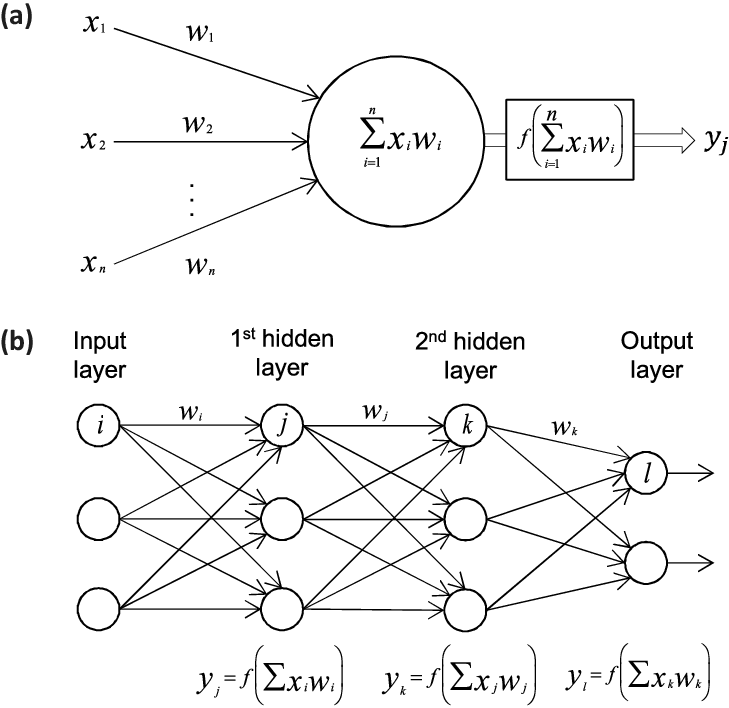
\includegraphics[width=0.5\textwidth]{images/tnn_ann.png}
    \caption{(a) Visualization of an artificial neuron from \cite{vieira2017using} depicting the output as a function of weighted sum of the inputs (equation \ref{eq:op_neuron}) (b). The artificial neural network consisting of the input layer, hidden layers and the output layer. Image from \cite{article}}
    \label{fig:mlp}
\end{figure}
The connections between the layers are feed-forward and uni-directional. The input layer serves as a buffer layer with no transformation of the input while in the other layers the neurons implement non-linear transfer functions on the weighted connections from the previous layer as shown in figure \ref{fig:mlp} (a), the output $y$ from the neuron can be expressed as:
\begin{equation}
    \label{eq:op_neuron}
    y = g(\sum_{i=1}^{N} w_i x_i +b) 
\end{equation}
where $w_i$ represents the weighting of the inputs and the b represents the bias for the neuron. Using the organizational structure, the neural network is able to learn complex transformations from the input data. In fact, It has been shown that an MLP with just one hidden layer and a finite number of neurons is able to act as a universal function approximator(\cite{universal_mlp}). Consider that we have an input vector in the N dimensional space and the output is needed in the M dimnensional space, then such an MLP (having non-linear transfer functional units) can implement any continuous mapping from the N dimensional space to the N dimensional space, with arbitrary accuracy. 

The network can be made 'deep' by adding additional hidden layers. It is employed in Neuroimaging studies in use-cases where there is a requirement to eliminate the need for manual feature selection.




\end{document}